

% !TeX spellcheck = en_US 
\documentclass[12pt,english]{report}
\usepackage{tesi}
% CORSO DI LAUREA:
\def\myCDL{Master in\\Computer Science}

% TITOLO REPORT:
\def\myTitle{Simulation \\
\large{Final report on Agent-Based Simulation for StiroApp}}

% AUTORE:
\def\myName{Samuele Simone}
\def\myMat{Matr. Nr. 11910A}

\def\myRefereeA{Prof. Alberto Ceselli}

% ANNO ACCADEMICO
\def\myYY{2022-2023}

% Il seguente comando introduce un elenco delle figure dopo l'indice (facoltativo)
%\figurespagetrue

% Il seguente comando introduce un elenco delle tabelle dopo l'indice (facoltativo)
%\tablespagetrue


% Package di formato
\usepackage[a4paper]{geometry}		% Formato del foglio
\usepackage[english]{babel}			% Supporto per l'italiano
\usepackage[utf8]{inputenc}			% Supporto per UTF-8
\usepackage[a-1b]{pdfx}			% File conforme allo standard PDF-A (obbligatorio per la consegna)

% Package per la grafica
\usepackage{graphicx}				% Funzioni avanzate per le immagini
\usepackage{hologo}					% Bibtex logo with \hologo{BibTeX}
%\usepackage{epsfig}				% Permette immagini in EPS
\usepackage{listings}
\usepackage{xcolor}
\usepackage{hyperref}

%Creating dark code theme for listings
\definecolor{codegreen}{rgb}{0.58,0.88,0.58}
\definecolor{codegray}{rgb}{0.5,0.5,0.5}
\definecolor{codeorange}{rgb}{0.72,0.54,0.45}
\definecolor{backcolour}{rgb}{0.10,0.13,0.14}
\definecolor{myorange}{RGB}{245,156,74}
\definecolor{keyw}{rgb}{0.60,0.85,0.98}
\lstdefinestyle{mystyle}{
    backgroundcolor=\color{backcolour},   
    commentstyle=\color{codegreen},
    keywordstyle=\color{keyw},
    numberstyle=\tiny\color{codegray},
    stringstyle=\color{codeorange},
    basicstyle=\ttfamily\footnotesize \color{white},
    breakatwhitespace=false,         
    breaklines=true,                 
    captionpos=b,                    
    keepspaces=true,                 
    numbers=left,                    
    numbersep=5pt,                  
    showspaces=false,                
    showstringspaces=false,
    showtabs=false,                  
    tabsize=2
}

\lstset{style=mystyle}

% Package tipografici
\usepackage{amssymb,amsmath,amsthm} % Simboli matematici
\usepackage{listings}				% Scrittura di codice

% Package ipertesto
\usepackage{url}					% Visualizza e rendere interattii gli URL
\usepackage{hyperref}				% Rende interattivi i collegamenti interni
\usepackage{notes2bib}

\usepackage{multirow}
\hypersetup{
    colorlinks=true,
    linkcolor=blue,
    urlcolor=myorange,
    filecolor=magenta,  
    }

\begin{document}

% Creazione automatica del frontespizio
\frontespizio
\beforepreface
\afterpreface


\chapter{Introduction}
ci

\chapter{Model}\label{ch:model}
In order to simulate the traffic over the app and to estimate revenues, costs and other KPI that are described in the Chapter \ref{ch:KPI}, I used the agent-based modeling.
As well described from the Columbia University website \cite{columbia}, Agent-based models are computer simulations used to study the interactions between people, things, places, and time. They are stochastic models built from the bottom up meaning individual agents (often people in epidemiology) are assigned certain attributes.The agents are programmed to behave and interact with other agents and the environment in certain ways. \par
The agents that are involved in the model are:
\begin{itemize}
\item \textbf{Worker\_iron}: Represents the worker within the application
\item \textbf{Buyer}: Represents the buyer, i.e., the one who creates the posts with their clothing
\item \textbf{Rider}: He is in charge of picking up the goods and delivering them to the respective worker/buyer.
\item \textbf{Scheduler}: He/she is in charge of handling incoming posts and directing them
\end{itemize}
We will see during this Chapter how I modeled these agents for StiroApp.
\section{Worker\_iron agent}
Below I will go on to describe the logic of the Worker\_iron agent. The technical details will be discussed in Chapter \ref{ch:implementation}.
Basically the worker as soon as it is generated waits for some order to be assigned to it, in a \textbf{Waiting state}. 
Through a branch the worker by condition wonders whether it has received the order or not. In the first case then he can start working by entering the \textbf{Working state} and after a Uniform Discrete random variable $\mathcal{U}(a,b)$ where $a = 2, b = 60$ minutes, he enter in a \textbf{ReadyForDelivery state} Then, with a 10 minutes Timeout transition enter in a branch and through a Bernoulli random variable $\mathcal{B}(p)$ where $p = 0.7$ he decides whether to finish his task or re-enter the \textbf{Waiting state}.In the second case, on the other hand, he enters the \textbf{Thinking state} and then after a small timeout point to the same transition branch where there is the Bernoulli random variable.
\section{Buyer agent}
The Buyer as soon as it is generated is in a \textbf{Waiting state}. In fact here, through a transition to the branch you want to check if that specific agent is new or already created and therefore is waiting for his order. If he is new then he can create a post with his clothing by entering the \textbf{CreatePost state}. After that through a Timeout of 10 min he enters the \textbf{Waiting state} and also through a Bernoulli random variable $\mathcal{B}(p)$ where $p = 0.7$ he decides whether to finish his task or re-enter the \textbf{Waiting state}. If,instead, he has already a pending order and it's notified as delivered he can again through the same branch if finish or re-enter.
\section{Rider agent}
The rider plays a key role within my simulation. In fact it involves a slightly more complex logic in that its task depends on the type of order received. Initially it is in a \textbf{Waiting state}. As soon as it receives an order it goes into the \textbf{AssignedOrder state}. Then it has to figure out through the properties of the received order whether it is a pickup or a delivery. In fact the rider first has to go to the buyer and receive the clothes for which it wants to perform a service and from there, the rider has to deliver it at the chosen worker. Once this is done through a Bernoulli random variable $\mathcal{B}(p)$ where $p = 0.7$ decides whether to continue working enter the Waiting state again or stop working. If it continues working it may happen to receive the delivery order and then go to a worker who is in the ReadyForDelivery state, pick up the clothes, and return them to the buyer who owns those clothes.
\section{Scheduler agent}
This agent, on the other hand, acts as a conduit between agents by handling the exchange of messages (specifically, we will see that we will be dealing with the dispatch of an object of type Post). It presents two states, a \textbf{Wait state} and a \textbf{Dispatch state}. It simply presents two transitions and allow you to manage the event queue and based on the type of post received sort the dispatches to the correct recipient.
\chapter{Implementation}\label{ch:implementation}
In practice to implement the models described above, I have used AnyLogic software.
Specifically in this chapter I will show the various flowcharts and the more specific transitions that require further study.
\section{Buyer agent implementation}
Let's start with the implementation of the Buyer.
\begin{figure}[hbtp]
\caption{Buyer statechart}
\centering
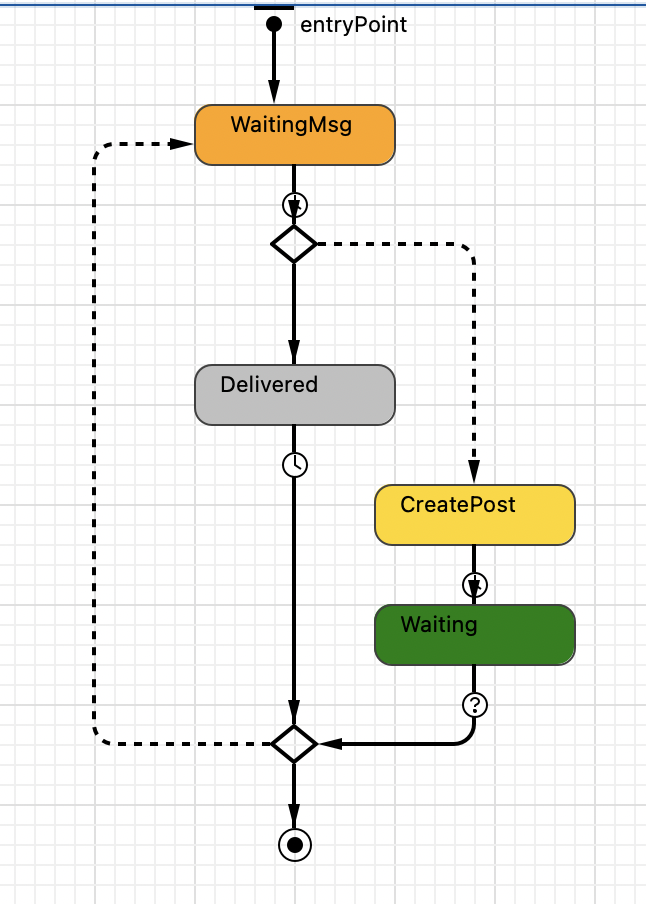
\includegraphics[scale=0.4]{../Images/buyerstatechart.png}
\end{figure}
The most important part to analyze is within the CreatePost state. In fact, there is some Java code here that is responsible for the operation of the orders.
\begin{lstlisting}[language=Java]
Post p = new Post();
p.buyer = this;
p.whoIs = 0;
p.numOfCloths = uniform_discr(1, 10);
p.postPrice = Math.round((uniform(0.5, 20) * p.numOfCloths) * 100.00) / 100.00;
post = p;
send(p, main.scheduler);
\end{lstlisting}
As you can see from the code I created a Post class where inside there are a number of attributes.
\begin{itemize}
\item \textbf{buyer}: who is the buyer and so in this case I pass him the \textbf{this} pointer, so himself being in the Buyer agent
\item \textbf{whoIs}: this is an integer attribute that allows me to figure out whether the order was placed by the Buyer (0) or the Worker (1)
\item \textbf{numOfCloths}: for the cloth numbers I relied on a Uniform Discrete random variable $\mathcal{U}$ of parameter $a = 1, b = 10$.
\item \textbf{postPrice}: same for post price by estimating on parameter b = 20
\item \textbf{status}: it's useful for understanding if the order is completed or is currently under working
\item \textbf{rider}: assign a rider for that specific post
\item \textbf{worker}: assign a worker for that specific post
\end{itemize}
This operation, on the other hand, must be commented out send(p, main.scheduler), since it is critical for handling the exchange of messages (and thus Posts).
Then the conditional transition are two: From the branch to delivered if the post (variable inside the Buyer agent) is not null and the status = 1.
\begin{lstlisting}
post != null && post.status ==  1
\end{lstlisting}
Same store from Waiting to the branch if status = 1.
\section{Scheduler agent implementation}
Another important agent is the Scheduler agent as we saw in the previous Chapter. However let's have a look inside the statechart.
\begin{figure}[hbtp]
\caption{Scheduler statechart}
\centering
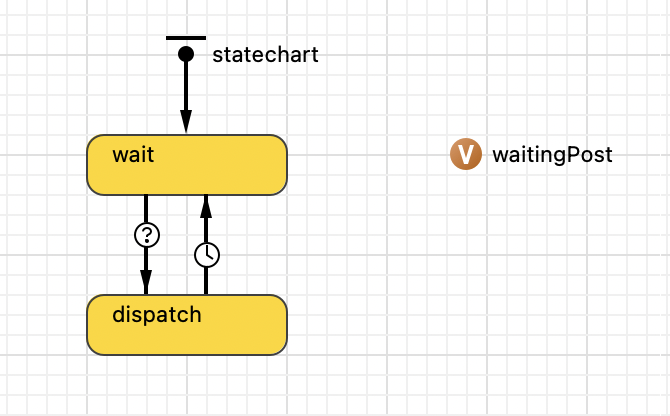
\includegraphics[scale=0.6]{../Images/schedulerstatechart.png}
\end{figure}
As you can see there are two transition in which one is conditional. Here the code for the trigger condition:
\begin{lstlisting}[language=Java]
waitingPost.size() > 0
\end{lstlisting}
so if the size of the queue isn't empty. Then if the condition is triggered there is this action to be executed:
\begin{lstlisting}[language=Java]
Post currPost = waitingPost.get(0);
waitingPost.remove(0);
if(currPost.whoIs == 0){
	Workers_iron w = main.workers_irons.findFirst(wi -> wi.inState(Workers_iron.Waiting));
	currPost.worker = w;
	Rider r = main.riders.findFirst(ri -> ri.inState(Rider.Waiting));
	if(r != null){
		currPost.rider = r;
		send(currPost,r);
	}
	
}else{
	Rider r = main.riders.findFirst(ri -> ri.inState(Rider.Waiting));
	if(r != null){
		currPost.rider = r;
		send(currPost,r);
	}
	
}
\end{lstlisting}
So I'll extract from the queue the first order and I remove it. Then I check if the order is from the Buyer, so it means that we need to search and find the first worker that is in the Waiting state, assign it to the Post attribute worker and the find the first rider that is in a Waiting state. If so, we assign the rider to the currentPost and then send currentPost to the rider. Instead, if the order is produced by the Worker, we just find a free rider that can take the processed order and send back to the Buyer. 
\section{Rider agent implementation}
In order to make the simulation work I need this agent. Here the statechart:
\begin{figure}[hbtp]
\caption{Rider statechart}
\centering
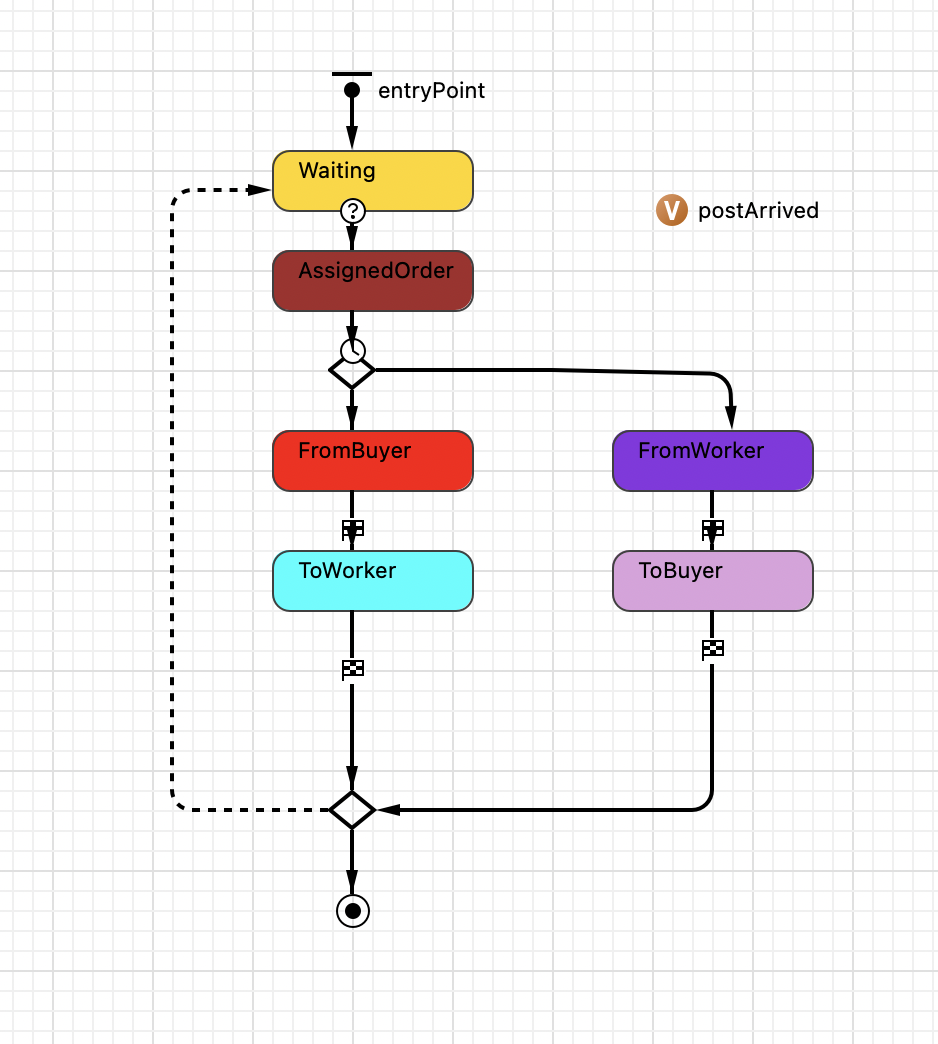
\includegraphics[scale=0.6]{../Images/riderstatechart.png}
\end{figure}
As we discussed previously the important thing here is to understand how the rider will move and how to trigger the conditions. Indeed we have two different flow: one is from \textbf{FromBuyer state} to \textbf{ToWorker state} state and here the rider will deliver the laundry from the Buyer to the Worker that need now to iron/wash his cloths. On the other hand we have the flow from \textbf{FromWorker state} to \textbf{ToBuyer state} that means that the Worker has finished his job and now the rider can catch the laundry and deliver to the owner (Buyer).
When the rider is the \textbf{AssignedOrder state} through the condition
\begin{lstlisting}[language=Java]
postArrived.whoIs == 0
\end{lstlisting} 
we execute this action 
\begin{lstlisting}[language=Java]
moveTo(postArrived.buyer);
\end{lstlisting} 
Note that each state block has his own color. That's useful to recognize in which state the rider enter during the simulation by change the shapeColor using this code:
\begin{lstlisting}[language=Java]
shapeBody.setFillColor(red);
\end{lstlisting} 
When the rider is arrived for example to the Buyer , he will pass in the other state like ToWorker state only by the transition that is trigger by agentArrival. (It is represented as a checkered flag). When this is true the action is the follow:
\begin{lstlisting}[language=Java]
moveTo(postArrived.worker); 
\end{lstlisting} 
Same story but in the opposite way for the other branch. After the deliver the rider will set the postArrived to null and with the Bernoulli random variable as discussed in the Model Chapter we can continue the flow.
\section{Worker agent implementation}
Then to complete the flow, we need the Worker agent that has the duty of complete the service that the Buyer asked. Here the statechart:
\begin{figure}[hbtp]
\caption{Worker\_iron statechart}
\centering
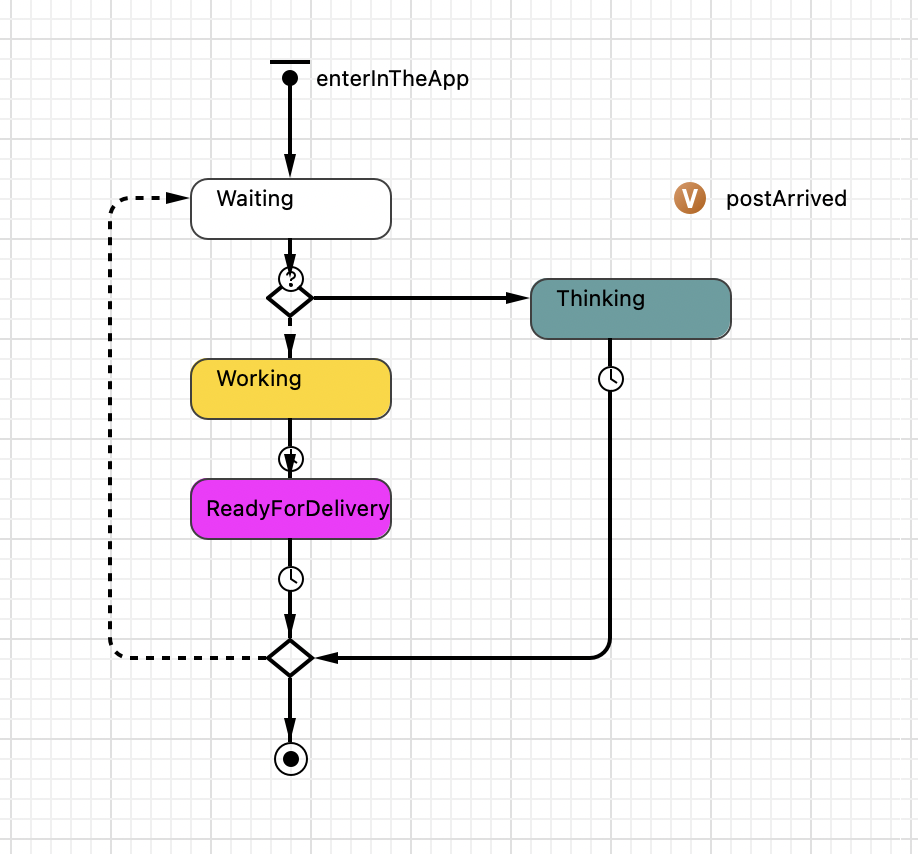
\includegraphics[scale=0.6]{../Images/workerstatechart.png}
\end{figure}
The only thing to discuss here is the conditional transition that allow us to enter inside the branch. Indeed:
\begin{lstlisting}[language=Java]
postArrived != null
\end{lstlisting} 
then the Worker can enter in the Working states otherwise he will enter in the Thinking state.
\section{Main agent implementation}
Finally let's talk about the special agent of the simulation that is called \textbf{Main agent}. It represents the "dashboard" of the simulation. 
\begin{figure}[hbtp]
\caption{Main agent }
\centering
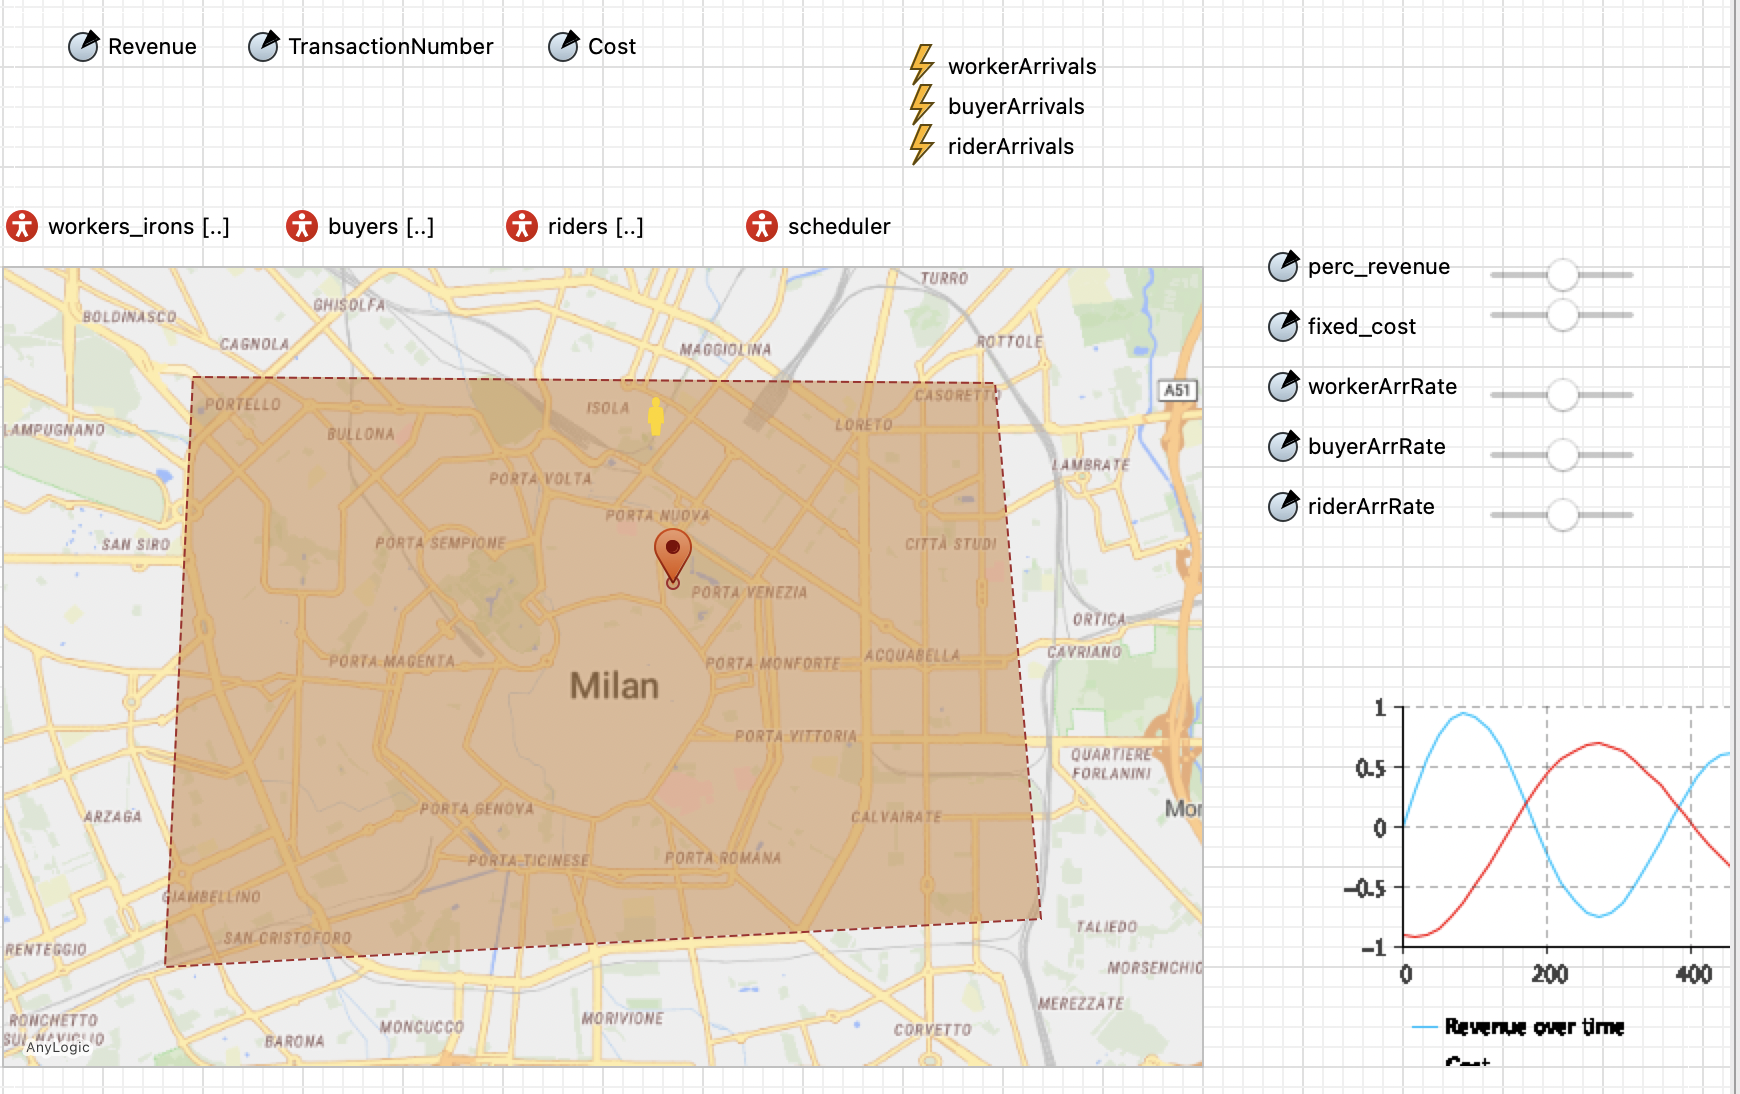
\includegraphics[scale=0.5]{../Images/main.png}
\end{figure}
As you can see the first thing that appear is the GIS map. It is centered in Milan, in which the simulation will run. With the help of the gis region I established a wide area within worker,buyer,rider can spawn. In the top-right corner there are 3 different arrivals, one for each agent, excluding the Scheduler.
With this code they can spawn in the GIS Region, just change the agent that we want to spawn:
\begin{lstlisting}[language=Java]
Rider r = add_riders();
Point p = gisRegion.randomPointInside();
Position q = new Position();
q.setLocation(p);
r.setPosition(q);
\end{lstlisting} 
Then let's consider the trigger type. They are all Rate and the amount is customizable with the sliders on the right side. Jusr riders are Rate/per day instead the other are Rate/per hours.
To conclude all are population of agents and just the scheduler is a single agent.

\chapter{KPI}\label{ch:KPI}
In the top of the Figure \ref{figure:main} there are 3 different parameters:
\begin{itemize}
\item Revenue
\item TransactionNumber
\item Cost
\end{itemize}
These are my KPI. The goal of this simulation is to maximize the Revenue KPI and compare it with the Cost KPI that I want to minimize. Indeed all the startup/industries wants to increase their productivity and their earnings by comparing it to the cost of all the infrastructure. 
The Revenue is counted when a valid transaction occurs. To be valid the flow Buyer $\rightarrow$ Worker and Worker $\rightarrow$ Buyer must be completed. Revenue and TransactionNumber are updated in the \textbf{ReadyForDelivery state} with the following code: 
\begin{lstlisting}[language=Java]
main.TransactionNumber++;
main.Revenue += postArrived.postPrice * main.perc_revenue + main.fixed_cost;
\end{lstlisting}
So,as described in the subsection \ref{subsection:businessModel}, I will use two parameters like perc\_revenue and  fixed\_cost in order to increase the earnings. So by playing with the sliders we obtain several different scenarios that are fully shown in the Chapter \ref{ch:experiments}.
\chapter{Experiments} \label{ch:experiments}
In this Chapter we will explore different scenarios obtained by changing parameters, number of population agents and we will try to maximize the Revenue as the KPI of the system.
\subsection{Original setup}
From the simulation panel I setup the simulation duration to 960 minutes that correspond to 16 hours. Then the other parameters:
\begin{itemize}
\item perc\_revenue : 0.15\%
\item fixed\_cost :0.20€
\item workerArrRate: 20 per hour
\item buyerArrRate: 20 per hour
\item riderArrRate: 10 per day
\end{itemize}
Here the results:
\begin{figure}[hbtp]
\caption{Original setup simulation}
\centering
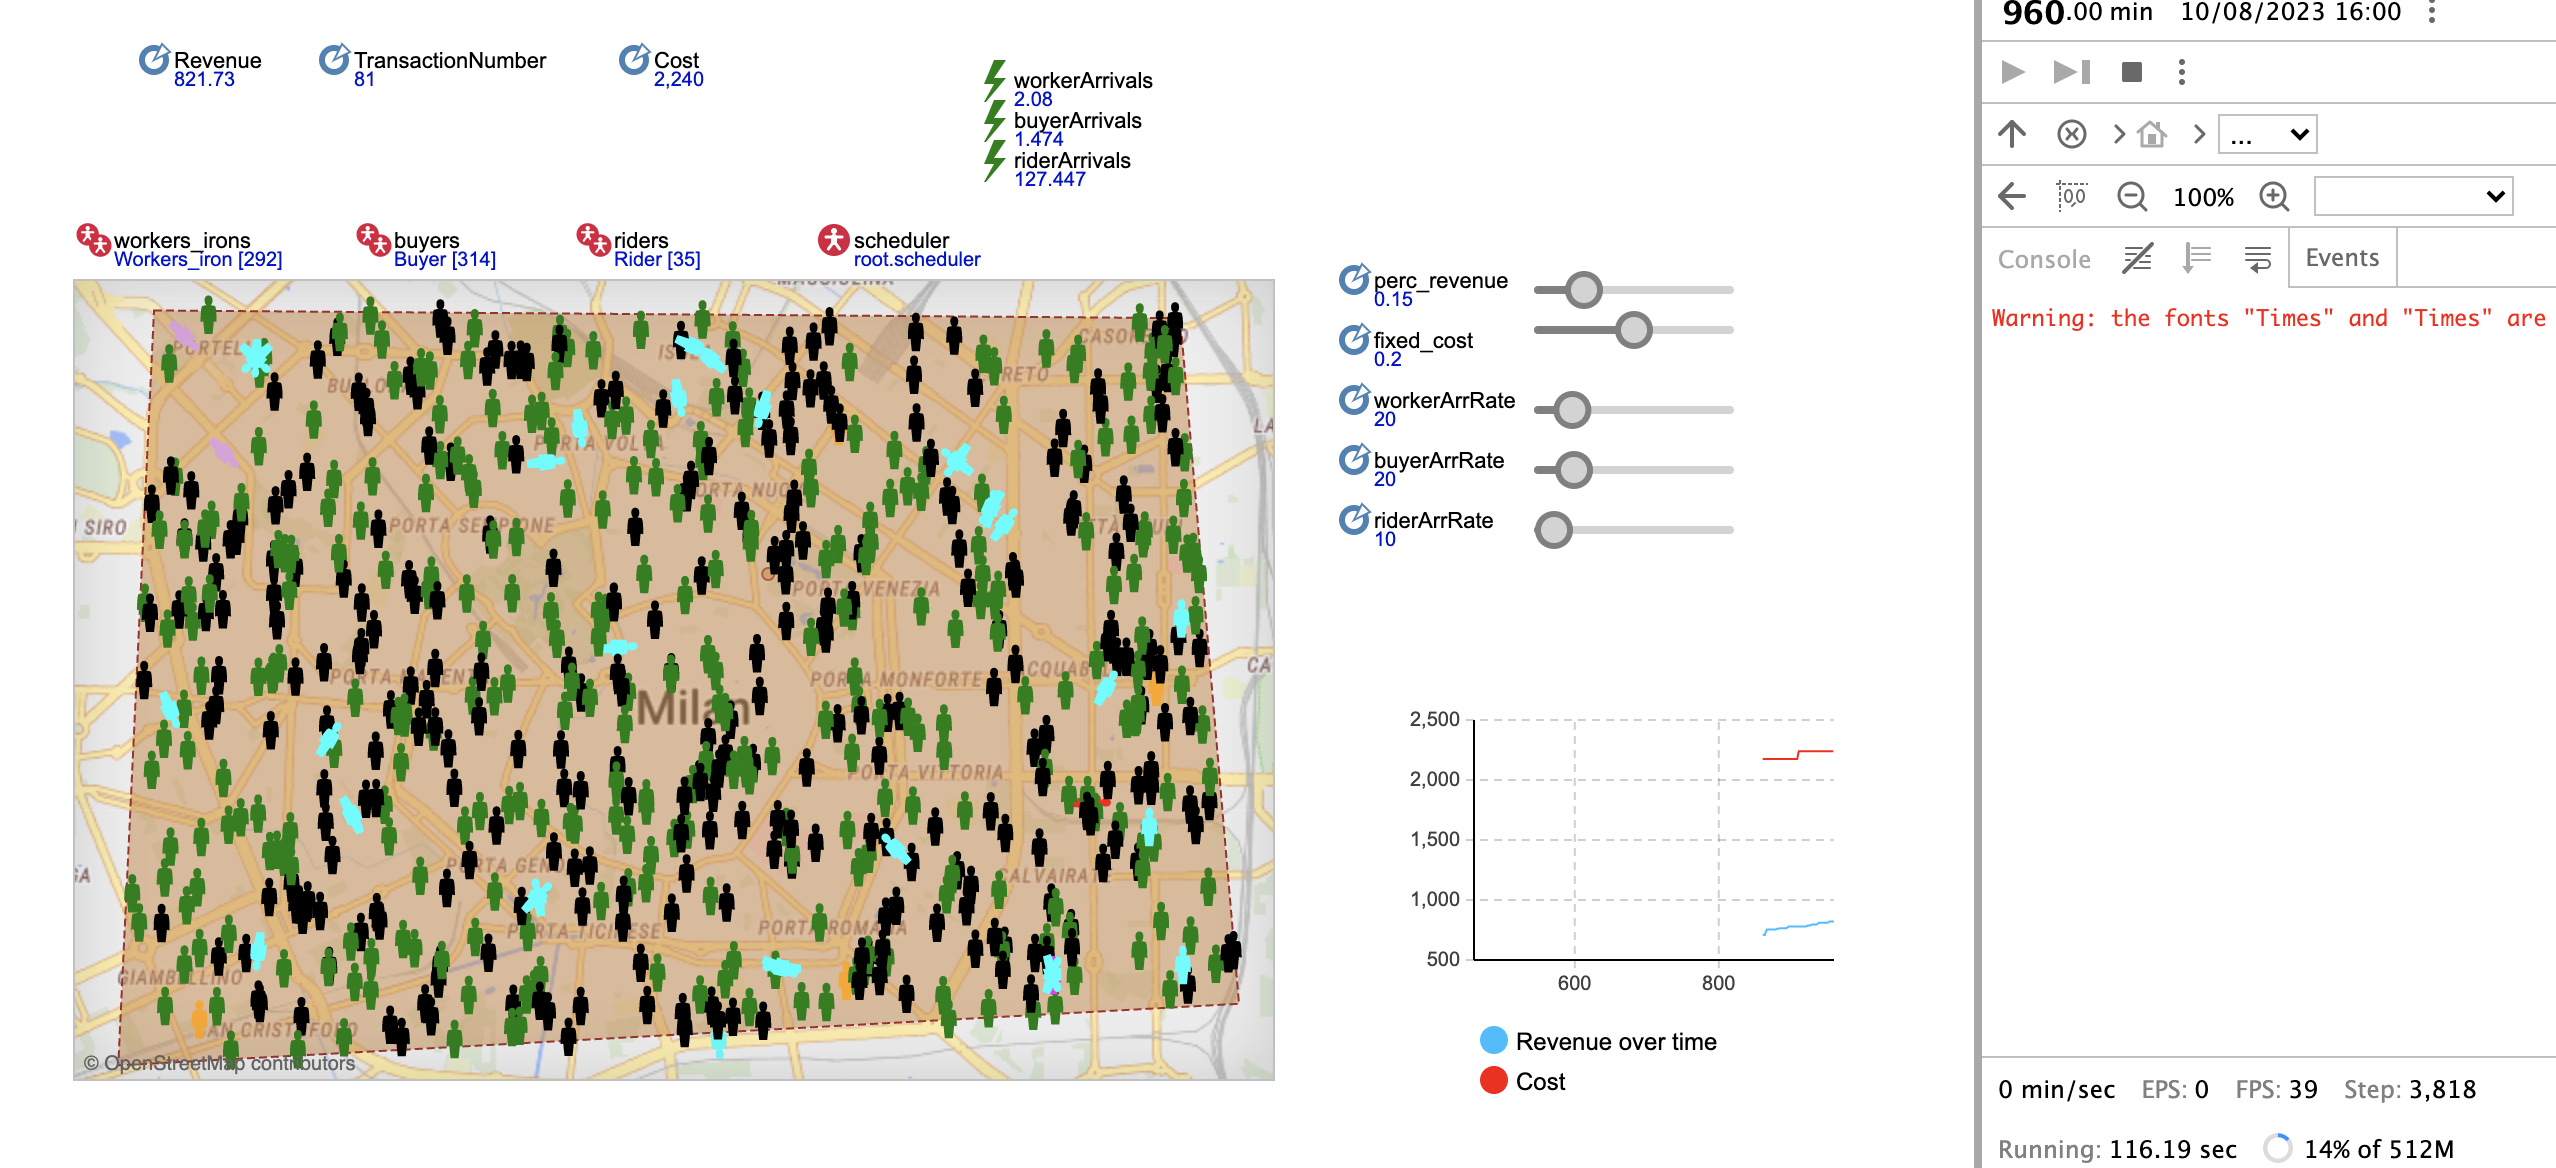
\includegraphics[scale=0.3]{../Images/sim01.png}
\end{figure}
As you can see from the top KPI or form the chart in the bottom-right side the Revenue are below the Cost. So there will be a lost over the first day. So we need to change some parameters and check if the situation will be better or not. For doing that I applied the What-If scenario different time as reported below.
\subsection{What-If scenario 1: }
\chapter{Conclusion}\label{ch:conclusion}
The purpose of this agent-based simulation was to validate a startup idea by going to simulate what are the possible scenarios so as to understand if the idea could actually be brought to market. From what can be gleaned, the business model presented is rather weak, in the sense that, it is a very good starting point to start making money. However, in order for the startup to cover the costs of maintaining infrastructure as well as personnel, it is necessary to complement this model with another one. In fact, the ideas could be:
\begin{itemize}
 \item Insertion of non-invasive advertising, between posts.
 \item In-app section of e-shop intended both for Workers for cleaning garments as well as for Buyers for maintaining garments.
 \item In-app purchase for premium packages (quality or speed) of the service.
 \end{itemize} 
In fact, what can be seen from the various experiments is that the cost of riders can be high and therefore a way must be sought through which maintaining riders is not such an intrusive problem. 
 Also, in the simulation approach, some simplifications were made for the purpose of getting straight to the point and trying to validate the logic behind the model. For example, the cost of clothes is assigned by a discrete uniform random variable where the parameter b is 20. This number could represent an underestimate of the model. So already by increasing that parameter the gains could grow.
 Certainly, both market analysis and business model analysis require a deeper and more detailed study by experts in the field. 
 In contrast, a simulated approach can give an idea of the feasibility of the service and experiment with different scenarios so as to maximize earnings.

%
%			BIBLIOGRAFIA
%

\bibliographystyle{unsrt}
\bibliography{bibliografia}
\addcontentsline{toc}{chapter}{Bibliografia}


\end{document}


 
